\subsection{法線ベクトルの計算}
境界上の積分を考える前に,外向き法線ベクトルの導出について説明する.
\begin{figure}[H]
  \centering
  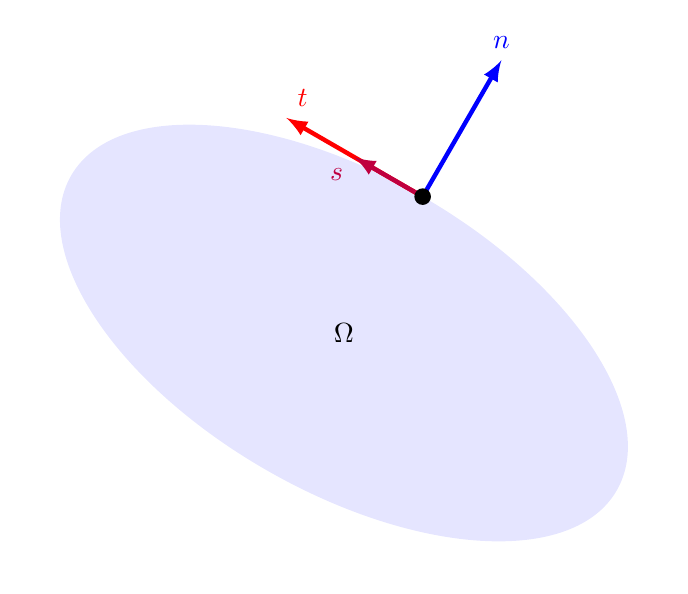
\begin{tikzpicture}
    % \draw[help lines] (0,0) grid (20,10);
    \fill[blue!10] (5,6)  ellipse [x radius=2cm, y radius=4cm, rotate=60];

    % 楕円上の点(x=7 のとき)
    \def\t{0} % t=0 のとき (右端の点) 
    \def\theta{60} % 楕円の回転角
    \def\a{2} % 長半径
    \def\b{4} % 短半径
    \def\cx{5} % 楕円の中心 x 座標
    \def\cy{6} % 楕円の中心 y 座標
    \def\scale{0.5} % ベクトルの縮小率を変更(0.5倍)
    % 点の座標計算
    \pgfmathsetmacro\xval{\cx + \a*cos(\t)*cos(\theta) - \b*sin(\t)*sin(\theta)}
    \pgfmathsetmacro\yval{\cy + \a*cos(\t)*sin(\theta) + \b*sin(\t)*cos(\theta)}
    % 接線ベクトル計算
    \pgfmathsetmacro\Tx{-\a*sin(\t)*cos(\theta) - \b*cos(\t)*sin(\theta)}
    \pgfmathsetmacro\Ty{-\a*sin(\t)*sin(\theta) + \b*cos(\t)*cos(\theta)}
    % 法線ベクトル計算(接線ベクトルを90度回転)
    \pgfmathsetmacro\Nx{\Ty}
    \pgfmathsetmacro\Ny{-\Tx}
    % 接線ベクトルの描画
    \draw[-{latex}, ultra thick, red] (\xval,\yval) -- ++(\scale*\Tx,\scale*\Ty) node[above right] {$\vect{t}$};
    \draw[-{latex}, ultra thick, purple] (\xval,\yval) -- ++(\scale*\scale*\Tx,\scale*\scale*\Ty) node[below left] {$\odif{\vect{s}}$};
    % 法線ベクトルの描画
    \draw[-{latex}, ultra thick, blue] (\xval,\yval) -- ++(\scale*\Nx,\scale*\Ny) node[above] {$\vect{n}$};
    % 点の描画
    \fill[black] (\xval,\yval) circle (3pt);
    \node at (5,6) {$\Omega$};
\end{tikzpicture}
\caption{境界上の点における法線ベクトルの導出}
\end{figure}
ここで,$\vect{t}$は単位接線ベクトル(Unit tangent vector),$\vect{n}$は単位法線ベクトル(Unit normal vector)である.$\vect{t}$は境界上の点の接線ベクトルであり,反時計周りを正とする.$\vect{n}$は$\vect{t}$に対して直角で,境界の外向きを正とする.
ベクトル$\odif{\vect{s}}$は次のように定義できる.
\begin{align}
  \odif{\vect{s}} &= \odif{x}\vect{e}_x + \odif{y}\vect{e}_y\\
  \odif{s} &= \sqrt{\odif{x}^2 + \odif{y}^2}
\end{align}
ここで,$\odif{x}$,$\odif{y}$は境界上の$\odif{\vect{s}}$に対応する変化量であり,$\vect{e}_x$,$\vect{e}_y$はそれぞれ$x$,$y$軸方向の単位ベクトルである.ここで,$\vect{t}$は$\odif{\vect{s}}$をその長さ$\odif{s}$で割ったものである.
\begin{equation}
  \vect{t} = \odv{x}{s}\vect{e}_x + \odv{y}{s}\vect{e}_y
\end{equation}
また,$\vect{n}$は次のように定義される.
\begin{equation}
  \vect{n} = n_x\vect{e}_x + n_y\vect{e}_y
\end{equation}
ここで$\vect{t}$に対して直角であるので,$\vect{t}$と$\vect{n}$の内積は$0$であり,$\vect{t}$と$\vect{n}$の外積は$\vect{e}_z$となる.
\begin{align}
  \label{Eq:tn-dot-product}
  \vect{t}\cdot\vect{n} &= n_x \odv{x}{s} + n_y \odv{y}{s} = 0\\
  \vect{t}\times\vect{n} &= \begin{vmatrix}
    \vect{e}_x & \vect{e}_y & \vect{e}_z\\
    \displaystyle\odv{x}{s} & \displaystyle\odv{y}{s} & 0\\
    n_x & n_y & 0
  \end{vmatrix}=\vect{e}_z\pab{n_x\odv{y}{s} - n_y\odv{x}{s}}=\vect{e}_z\notag\\
  \label{Eq:tn-cross-product}
  &n_x\odv{y}{s} - n_y\odv{x}{s} = 1
\end{align}
\eqref{Eq:tn-dot-product}式と\eqref{Eq:tn-cross-product}式を連立して解くと,最終的に次式を得る.
\begin{equation}
  \vect{n}=\odv{y}{s}\vect{e}_x - \odv{x}{s}\vect{e}_y
\end{equation}